\documentclass[11pt]{beamer}
\usepackage[utf8]{inputenc}
\usepackage[T1]{fontenc}
\usepackage{lmodern}
\usepackage{tikz}
\usetikzlibrary{3d, shapes.geometric,automata, shapes, arrows.meta, positioning, fit, calc, backgrounds}

\tikzstyle{block} = [rectangle, draw, fill=blue!20, text centered, rounded corners, minimum height=2em]
\tikzstyle{line} = [draw, -Stealth]
\tikzstyle{container} = [draw, rectangle, dashed, inner sep=0.7em]

 \usepackage{graphicx}
\usetheme{CambridgeUS}
\begin{document}
	\author{Emmanuel Adjei\\
	University of California, Irvine\\
	Statistics Department (DHB 2011)}
	\title{
		The Mathematical Principles Behind OpenAI's SORA }
	%\subtitle{}
	%\logo{}
	%\institute{}
	%\date{}
	%\subject{}
	%\setbeamercovered{transparent}
	%\setbeamertemplate{navigation symbols}{}
	\begin{frame}[plain]
		\maketitle
	\end{frame}
	
	\begin{frame}
		\frametitle{OUTLINE}
		\begin{itemize}
			\item Introduction
			\item Methodology
			\begin{enumerate}
				\item Diffusion Probabilistic Modeling
				\item Scalable Diffusion Models with Transformer
				\item Tubelet embedding
				\item Factorized dot-product attention mechanism
				
			\end{enumerate}
			\item Reference
		\end{itemize}
	\end{frame}

\begin{frame}
	\frametitle{Introduction}
	
	\begin{figure}
		\centering
		\includegraphics[width=0.75\linewidth]{aaa.png} 
	\caption{Source:https://images.app.goo.gl/3cC34WCaGwAApw9o9}
		\label{fig: Source: https://images.app.goo.gl/3cC34WCaGwAApw9o9} % Changed the label to a proper one
	\end{figure}
	Everyone has witnessed the unveiling of Sora, OpenAI's remarkable video generation tool. 
	
\end{frame}

\begin{frame}
	\frametitle{Introduction}
\begin{itemize}
	\item Advancing from DALL·E's static imagery, this innovation adds a vibrant, dynamic layer, reshaping our engagement with AI-generated material. The inevitable inquiry emerges: how did OpenAI accomplish this breakthrough?
	\item In this presentation we will delve into the mathematics and framework that form the background  for this model. 
\end{itemize}
		
\end{frame}




\begin{frame}
	\begin{block}{Methodology}
	Diffusion Probabilistic Modeling.
	\end{block}
	
	\begin{figure}
		\centering
		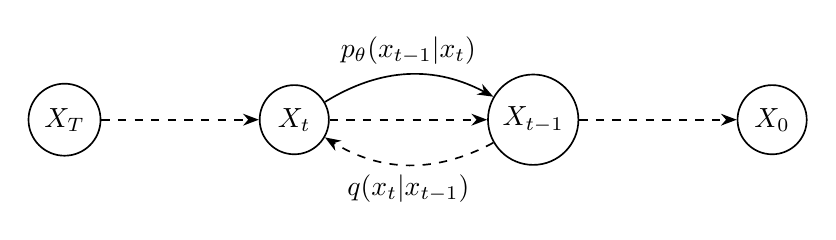
\begin{tikzpicture}[->, >=Stealth, auto, semithick, node distance=2cm]
			\node[state] (XT) {$X_T$};
			\node[state] (Xt) [right=of XT] {$X_t$};
			\node[state] (Xtm1) [right=of Xt] {$X_{t-1}$};
			\node[state] (X0) [right=of Xtm1] {$X_0$};
			
			\path
			(XT) edge[dashed] (Xt)
			(Xt) edge[dashed] (Xtm1)
			(Xtm1) edge[dashed] (X0)
			(Xt) edge[bend left] node[above] {$p_{\theta}(x_{t-1}|x_t)$} (Xtm1)
			(Xtm1) edge[bend left,dashed] node[below] {$q(x_t|x_{t-1})$} (Xt);
		\end{tikzpicture}
		\caption{The directed graphical model}
	\end{figure}
A diffusion probabilistic model is a Markov chain with parameters that is trained through variational inference to generate samples that resemble the data within a finite time frame.
\end{frame}


\begin{frame}
	\frametitle{Diffusion Probabilistic Modeling.}
The given model defines \( p_\theta(\mathbf{x}_0) \) as the integral of \( p_\theta(\mathbf{x}_{0:T}) \) over \( \mathbf{x}_{1:T} \), where \( \mathbf{x}_1, \ldots, \mathbf{x}_T \) are latent variables with the same dimensionality as the data \( \mathbf{x}_0 \), which is distributed according to \( q(\mathbf{x}_0) \). The joint distribution \( p_\theta(\mathbf{x}_{0:T}) \) is denoted as the reverse process, characterized as a Markov chain with learned Gaussian transitions, beginning from \( p(\mathbf{x}_T) = \mathcal{N}(\mathbf{x}_T; \mathbf{0}, \mathbf{I}) \):

$$
p_\theta\left(\mathbf{x}_{0: T}\right):=p\left(\mathbf{x}_T\right) \prod_{t=1}^T p_\theta\left(\mathbf{x}_{t-1} \mid \mathbf{x}_t\right), \quad p_\theta\left(\mathbf{x}_{t-1} \mid \mathbf{x}_t\right):=\mathcal{N}\left(\mathbf{x}_{t-1} ; \boldsymbol{\mu}_\theta\left(\mathbf{x}_t, t\right), \mathbf{\Sigma}_\theta\left(\mathbf{x}_t, t\right)\right)
$$

$$
q\left(\mathbf{x}_{1: T} \mid \mathbf{x}_0\right):=\prod_{t=1}^T q\left(\mathbf{x}_t \mid \mathbf{x}_{t-1}\right), \quad q\left(\mathbf{x}_t \mid \mathbf{x}_{t-1}\right):=\mathcal{N}\left(\mathbf{x}_t ; \sqrt{1-\beta_t} \mathbf{x}_{t-1}, \beta_t \mathbf{I}\right)
$$
\end{frame}


\begin{frame}
	\frametitle{Scalable Diffusion Models with Transformer}
	
\begin{figure}
	\centering
	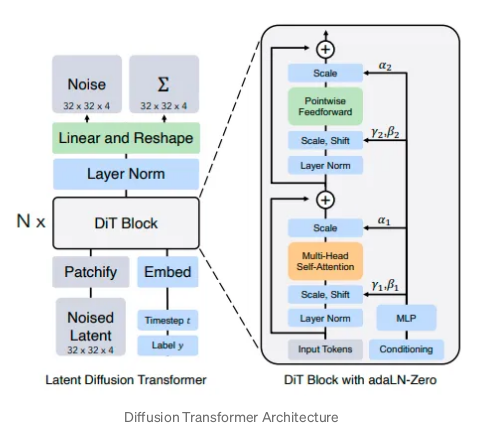
\includegraphics[width=0.55\linewidth]{dit.png} 
	\caption{Source:https://images.app.goo.gl/3cC34}
	\label{fig: Source: https://images.app.goo.gl/3cC34WCaGwAApw9o9} % Changed the label to a proper one
\end{figure}

\end{frame}

\begin{frame}
	\frametitle{Scalable Diffusion Models with Transformer}
	
The architecture is designed to handle the diffusion process in a transformer-based framework, likely aiming to leverage the transformer's ability to model long-range dependencies for generating or denoising data in a manner similar to denoising autoencoders but with the benefits of attention mechanisms. Nevertheless, transformers are highly resource-intensive, making them impractical for video scaling if we merely extend the temporal dimension.
\end{frame}


\begin{frame}
	\frametitle{Tubelet embedding}
	
	\begin{figure}
		\centering
		\includegraphics[width=0.43\linewidth]{ar.png} 
		\caption{Source:https://images.app.goo.gl/3cC34WCa}
		\label{fig: Source: https://images.app.goo.gl/3cC34WCaGwAApw9o9} % Changed the label to a proper one
	\end{figure}
	The key advantage of tubelet embedding is that it allows a neural network, such as a transformer, to process videos by taking into account the dynamic changes across frames, which is essential for tasks such as action recognition, video classification, or any other application requiring an understanding of both spatial and temporal dimensions of the video. This extract non-overlapping, spatio-temporal “tubes” from the input volume, and to linearly project this to $\mathbb{R}^d$ [1].
\end{frame}

\begin{frame}
	\frametitle{Factorized dot-product attention mechanism}
	
	
\begin{figure}
	\centering
	\includegraphics[width=0.85\linewidth]{las.png} 
	\caption{Source:https://images.app.goo.gl}
	\label{fig: Source: https://images.app.goo.gl/} % Changed the label to a proper one
\end{figure}
\end{frame}

\begin{frame}
	\frametitle{Factorized dot-product attention mechanism}
	By factorizing the attention this way, the model can efficiently process video data by treating space and time separately, which is computationally less demanding than the traditional method that would consider all spatial and temporal elements together. This also allows the model to specialize in extracting spatial features (like shapes and textures) and temporal features (like movement and change) from the video data, possibly leading to a more nuanced understanding and better performance on video-related tasks.
\end{frame}

\begin{frame}

	\begin{thebibliography}{100}
	
	\bibitem{} 
	Vivit: A video vision transformer,
		Arnab, Anurag and Dehghani, Mostafa and Heigold, Georg and Sun, Chen and Lu{\v{c}}i{\'c}, Mario and Schmid, Cordelia,
	Proceedings of the IEEE/CVF international conference on computer vision,
		6836--6846,
		2021

	   
	\bibitem{}  Denoising diffusion probabilistic models,
	   	Ho, Jonathan and Jain, Ajay and Abbeel, Pieter,
	   Advances in neural information processing systems,
	   33,
	   	6840--6851,
	   	2020
	 
\end{thebibliography} 
\end{frame}

\begin{frame}
	\begin{figure}
		\centering
		\includegraphics[width=0.93\linewidth]{tu.png} 
	\end{figure}

\end{frame}
\end{document}